\documentclass[a4paper,11pt]{article}


\usepackage{color}
\usepackage{array}
\usepackage{amsmath,amssymb}
\usepackage{graphics}
\usepackage[utf8]{inputenc}
\usepackage[spanish]{babel}


\addtolength{\textwidth}{2cm}
\addtolength{\hoffset}{-1cm}


\title{QSudoku}
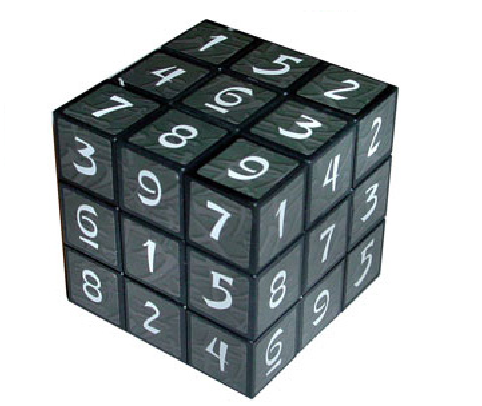
\includegraphics{sudo.png}


\title{Qsudoku}
\author{Ramón Carrillo, Juan Mite, Esteban Muñoz}

\begin{document}
\maketitle
\tableofcontents

\section{Introducción}
Es una aplicación realizada en lenguaje c++, utilizando el IDE Qt Creator, es una adaptación de famoso Sudoku, un pasatiempo que se publicó por primera vez a finales de la década de 1970 y se popularizó en Japón en 1986, dándose a conocer en el ámbito internacional en 2005 cuando numerosos periódicos empezaron a publicarlo en su sección de pasatiempos.

\subsection{Descripción}
El objetivo del sudoku es rellenar una cuadrícula de 9 x 9 celdas (81 casillas) dividida en subcuadrículas de 3 x 3 (también llamadas "cajas" o "regiones") con las cifras del 1 al 9 partiendo de algunos números ya dispuestos en algunas de las celdas. Aunque se podrían usar colores, letras, figuras, se conviene en usar números para mayor claridad, lo que importa, es que sean nueve elementos diferenciados, que no se deben repetir en una misma fila, columna o subcuadrícula. Un sudoku está bien planteado si la solución es única. La solución de un sudoku siempre es un cuadrado latino, aunque el recíproco en general no es cierto ya que el sudoku establece la restricción añadida de que no se puede repetir un mismo número en una región. 

\section{Manual de usuario} 


\subsection{Pasos de la aplicación}
Al lanzar la aplicación se mostrará una pantalla de inicio la cual permitirá al jugador registrarse, escoger la dificultad de juego, ver las estadísticas de juegos pasados, desarrolladores e iniciar su juego con los requisitos que especificó al inicio.

\subsection{Pantalla inicial}
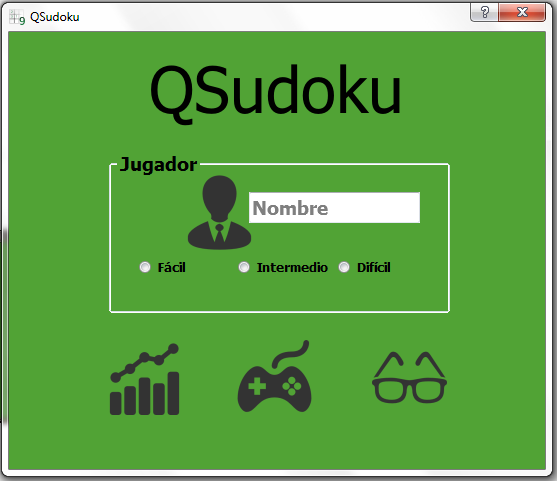
\includegraphics{inicio.png}

Ventana que se lanza al iniciar el juego.
\subsection{Preferencias}
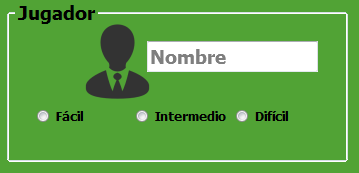
\includegraphics{nombre.png}

Aquí el jugador dejará su nombre y escogerá la dificultad con la que quiera fijar el tablero, si el jugador no fija una dificultad, el juego le asigna una facil por default.
\subsection{Juego nuevo}

\includegraphics{nuevoICO.png}

Al presionar aquí el jugador empezará con el juego.
\subsection{Estadísticas}

\includegraphics{estadistICO.png}

Al presionar aquí el jugador verá las estadisticas.

\subsection{Desarrolladores}

\includegraphics{develoICO.png}

Al presionar aquí el jugador verá información de los desarrolladores.


\subsection{Botón Home}

\includegraphics{home.png}

Al presionar aquí el jugador regresará a la pantalla de inicio.

\section{Ventanas}


\subsection{Juego Nuevo}
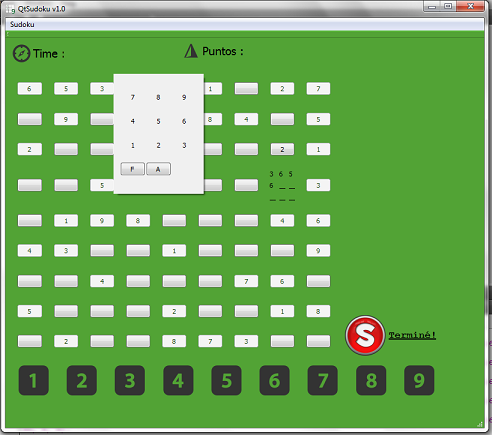
\includegraphics{tablero.png}
\subsection{Barra de menú}
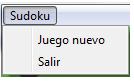
\includegraphics{barra.png}

En este menú el jugador contará con dos opciones, la funcionalidad de las mismas se detalla a continuación.
\subsection{Sudoku /Juego Nuevo}
El jugador podrá llenar un nuevo tablero, es decir reiniciar la parida desde Cero.
\subsection{Sudoku /Salir}
El jugador podrá salir del juego dando clic aquí, lo hará sin guardar partida simplemente cancelará su juego.
\subsection{Botón Terminé!}

\includegraphics{termine.png}

Al presionar aquí el jugador comprobará si llenó su tablero correctamente o no.
\subsection{Desarrolladores}
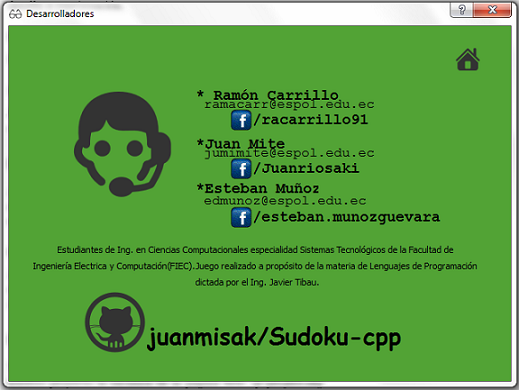
\includegraphics{pagdesa.png}

Aquí se muestra información acerca del juego como por ejemplo la versión del juego, desarrolladores, ubicación del repositorio Git Hub y la dirección de facebook de cada uno de ellos.
Juan Mite, Daniel Muñoz, Ramón Carrillo, Estudiantes de la Escuela Superior Politécnica del Litoral a propósito de la materia de Lenguajes de programación dictada por el Ing. Javier Tibau profesor de la Facultad de Ingeniería Eléctrica y Computación.  
\subsection{Estadísticas}
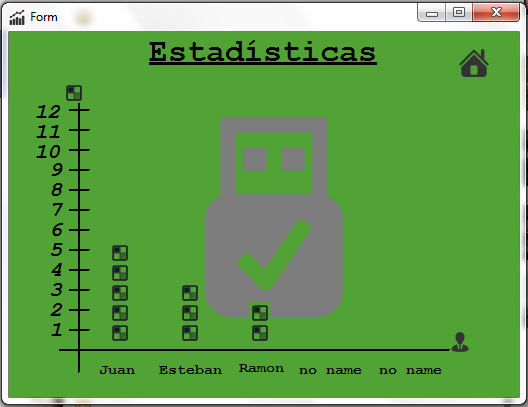
\includegraphics{estadist.png}

En esta ventana el jugador verá las puntuaciones de los 5 jugadores que han obtenido las mejores puntuaciones, en la esquina superior derecha hay un botón que lo reresará al Home.



\section{Bibliografía}
Toda la ayuda e información sobre de las herramientas que necesitamos para desarrollar nuestro proyecto la sacamos de la pagina web:
qt-project.org
\section{Referencias}
http://www.fceia.unr.edu.ar/lcc/cdrom/Instalaciones/LaTex/latex.html


\end{document}

